\documentclass[a4paper,12pt]{article} 

%%% Работа с русским языком
\usepackage{cmap}					% поиск в PDF
\usepackage{mathtext} 				% русские буквы в фомулах
\usepackage[T2A]{fontenc}			% кодировка
\usepackage[utf8]{inputenc}			% кодировка исходного текста
\usepackage[english,russian]{babel}	% локализация и переносы

%%% Дополнительная работа с математикой
\usepackage{amsmath,amsfonts,amssymb,amsthm,mathtools, gensymb} % AMS
\usepackage{icomma} % "Умная" запятая: $0,2$    ф--- число, $0, 2$ --- перечисление

%%Таблица
\usepackage[table,xcdraw]{xcolor}
\usepackage{caption}
\usepackage{floatrow}
\floatsetup[table]{capposition=top}
\floatsetup[wrapfigure]{capposition=bottom}
\usepackage{multirow}

\usepackage{hyperref}

%Отступы и поля 
\textwidth=18cm
\oddsidemargin=-1cm
\topmargin=-2cm
\textheight=25cm


%% Номера формул
\mathtoolsset{showonlyrefs=false} % Показывать номера только у тех формул, на которые есть \ref{} в тексте.

%% Шрифты
\usepackage{euscript}	 % Шрифт Евклид
\usepackage{mathrsfs} % Красивый матшрифт

%% Свои команды
\DeclareMathOperator{\sgn}{\mathop{sgn}}

%% Перенос знаков в формулах (по Львовскому)
\newcommand*{\hm}[1]{#1\nobreak\discretionary{}
{\hbox{$\mathsurround=0pt #1$}}{}}

%% Стиль страницы
\usepackage{fancyhdr}

%% Для рисунков
\usepackage{graphicx}
\usepackage[export]{adjustbox}
\usepackage{float}
\usepackage{ragged2e}
\usepackage{wrapfig}

\pagestyle{fancy}
\begin{document}
\begin{titlepage}
\begin{center}
%\vspace*{1cm}
\large{\small ФЕДЕРАЛЬНОЕ ГОСУДАРСТВЕННОЕ АВТОНОМНОЕ ОБРАЗОВАТЕЛЬНОЕ\\ УЧРЕЖДЕНИЕ ВЫСШЕГО ОБРАЗОВАНИЯ \\ МОСКОВСКИЙ ФИЗИКО-ТЕХНИЧЕСКИЙ ИНСТИТУТ\\ (НАЦИОНАЛЬНЫЙ ИССЛЕДОВАТЕЛЬСКИЙ УНИВЕРСИТЕТ)\\ ФАКУЛЬТЕТ АЭРОКОСМИЧЕСКИХ ТЕХНОЛОГИЙ}
\vfill
\line(1,0){490}\\[1mm]
\huge{Лабораторная работа 1.3}\\
\huge\textbf{Изучение рассеяния медленных электронов на атомах (эффект Рамзауэра)}\\
\line(1,0){490}\\[1mm]
\vfill
\begin{flushright}
\normalsize{Рогозин Владимир}\\
\normalsize{\textbf{Группа Б03-106}}\\
\end{flushright}
\end{center}
\end{titlepage}
\fancyhead[L] {Работа 1.3}

\textbf{Цель работы}:
исследовать энергетическую зависимость вероятности рассеяния электронов атомами инертного газа, определить энергии электронов, при которых наблюдается «просветление» ксенона, и оценить размер его внешней электронной оболочки.


% \textbf{Оборудование}:
% лазер; кассета с набором сеток разного
% периода; линзы; щель с микрометрическим винтом; оптический стол
% c набором рейтеров и крепёжных винтов; экран; линейка.


\section{Теоретические сведения}
К. Рамзауэр в 1921 г. исследовал зависимость поперечных сечений упругого рассеяния электронов (с энергией до 10 эВ) на атомах аргона. В результате этих исследований было обнаружено явление, получившее название \textit{эффекта Рамзауэра}.

\begin{wrapfigure}[17]{r}{0.4\textwidth}\label{fig: Scattering in Ramsauer–Townsend experiment}
    \begin{center}
    \vspace{-20pt}
        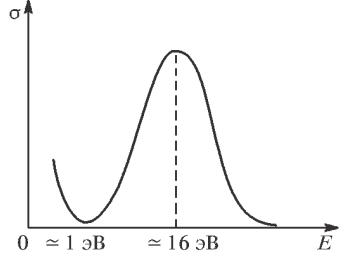
\includegraphics[width = 0.9\textwidth]{Scattering in Ramsauer–Townsend experiment.png}
    \end{center}
    \caption{Качественная картина измерения результатов упругого рассеяния электронов в аргоне}
\end{wrapfigure}
Эффективное сечение реакции (иногда его называют поперечным сечением или просто сечением реакции) -- это величина, характеризующая вероятность перехода системы двух сталкивающихся частиц в результате их рассеяния (упругого или неупругого) в определенное конечное состояние. Сечение $\sigma$ равно отношению числа $N$ таких переходов в единицу времени к плотности $nv$ потока рассеиваемых частиц, падающих на мишень, т. е. к числу частиц, проходящих в единицу времени через единичную площадку, перпендикулярную к их скорости $v$ ($n$ -- плотность числа падающих частиц)

\begin{equation}\label{eq: sigma}
    \sigma = \frac{N}{nv}.
\end{equation}
Таким образом, сечение имеет размерность площади.

Качественно результат экспериментов Рамзауэра при энергии электронов порядка десятков электрон-вольт на аргоне рассеяния электронов в аргоне
показан на рис. \hyperref[fig: Scattering in Ramsauer–Townsend experiment]{1}. По мере уменьшения энергии электрона от нескольких десятков электрон-вольт поперечное сечение его упругого рассеяния растет, как это и следует из очень простых рассуждений: чем меньше скорость электрона, тем медленнее он «проскакивает» мимо атома, тем больше время взаимодействия электронов с атомом и, тем самым, больше вероятность этого взаимодействия, т. е. сечение реакции. Однако в эксперименте наблюдалось, что при энергиях меньше $16$ эВ сечение начинает уменьшаться, а при $E \approx 1$ эВ практически равно нулю, т. е. аргон становится прозрачным для электронов. При дальнейшем уменьшении энергии электронов сечение рассеяния опять начинает возрастать.

Такое поведение электронов нельзя объяснить с позиций классической физики.

С точки зрения квантовой теории картина рассеяния выглядит следующим образом. Внутри атома потенциальная энергия налетающего электрона $U$ отлична от нуля, скорость электрона изменяется, становясь равной $v'$ соответствии с законом сохранения энергии
\begin{equation}\label{eq: Energy conservation law}
    E = \frac{mv^2}{2} = \frac{mv'^2}{2} + U, 
\end{equation}
а значит, изменяется и длина его волны де Бройля. Таким образом, по отношению к электронной волне атом ведет себя как преломляющая среда с относительным показателем преломления
\begin{equation}\label{eq: Refractive index}
    n = \frac{\lambda}{\lambda'} = \sqrt{1 - \frac{U}{E}}.
\end{equation}
Решение задачи о рассеянии электрона на сферической потенциальной яме достаточно громоздко, поэтому для качественного анализа вопроса рассмотрим более грубую модель: будем считать, что электрон рассеивается на одномерной потенциальной яме конечной глубины. Форму реального потенциала для качественных оценок можно считать прямоугольной. Модель прямоугольной потенциальной ямы является хорошим приближением для атомов тяжелых инертных газов, отличающихся наиболее компактной структурой и резкой внешней границей.

Уравнение Шредингера в данном случае имеет вид

\begin{equation}\label{eq: Shroedenger equation}
    \psi'' + k^2\psi = 0,\; \text{ где } 
    k^2 = 
    \begin{cases}
        k_1^2 = \frac{2mE}{\hbar^2}& \text{ -- в областях  I, III}, \\
        k_2^2 = \frac{2m(E + U_0)}{\hbar^2}& \text{ -- в области II}. \\
    \end{cases} 
\end{equation}
Коэффициент прохождения равен отношению квадратов амплитуд прошедшей и падающей волн и определяется выражением
\begin{equation}\label{eq: Transmission coefficient}
    D = \frac{16k_1^2 k_2^2}{16k_1^2 k_2^2 + 4(k_1^2 - k_2^2)^2\sin^2(k_2l)}
\end{equation}

\begin{figure}[H]\label{fig: Potential well scheme}
    \centering
    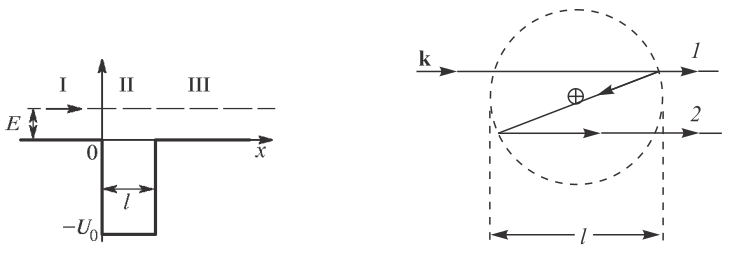
\includegraphics[width = 0.9\textwidth]{Potential well.png}
    \caption{Слева -- схематическое изображение прямоугольной ямы, над которой пролетает частица с энергией $E$, справа -- схема интерференции волн де Бройля при рассеянии на атоме}
\end{figure}

Коэффициент прохождения частицы над ямой имеет, в зависимости от её энергии, ряд чередующихся максимумов и минимумов. В частности, если $k_2l = \pi$, то коэффициент прохождения равен единице, т. е. отраженная волна отсутствует, и электрон беспрепятственно проходит через атом, что является квантовым аналогом просветления оптики.

Таким образом, коэффициент прохождения электронов максимален при условии
\begin{equation}\label{eq: Max condition via n}
    k_2l = \sqrt{\frac{2m(E + U_0)}{\hbar^2}}l = n\pi,\;\; n = 1, 2, 3...
\end{equation}

то условие легко получить, рассматривая интерференцию электронных волн де Бройля в атоме. Движущемуся электрону соответствует волна де Бройля, длина которой определяется соотношением $\lambda = h/mv$. Если кинетическая энергия электрона невелика, то $E = mv^2 / 2$ и $\lambda = h / \sqrt{2mE}$. При движении электрона через атом длина волны де Бройля становится меньше и равна $\lambda' = h / \sqrt{2m(E + U_0)}$, где $U_0$ -- глубина атомного потенциала. При этом, как показано на рис. \hyperref[fig: Potential well scheme]{2} справа, волна де Бройля отражается от границ атомного потенциала, т. е. от поверхности атома, и происходит интерференция прошедшей через атом волны $1$ и волны $2$, отраженной от передней и задней границы атома (эти волны когерентны). 

Прошедшая волна $1$ усилится волной $2$, если геометрическая разность хода между ними $\Delta = 2l = \lambda'$ , что соответствует условию первого интерференционного максимума, т. е. при условии
\begin{equation}\label{eq: Max condition}
    2l = \frac{h}{\sqrt{2m(E_1 + U_0)}}.
\end{equation}
Здесь $E_1$ -- энергия электрона, соответствующая этому условию.

С другой стороны, прошедшая волна ослабится, если $\Delta = 2l = (3/2)\lambda'$ (условие первого интерференционного минимума), т. е. при
условии
\begin{equation}\label{eq: Min condition}
    2l = \frac{3}{2}\frac{h}{\sqrt{2m(E_2 + U_0)}}.
\end{equation}
Решая совместно уравнения \eqref{eq: Max condition} и \eqref{eq: Min condition}, можно исключить $U_0$ и найти эффективный размер атома $l$
\begin{equation}\label{eq: Atom diameter}
    l = \frac{h\sqrt{5}}{\sqrt{32m(E_2 - E_1)}}.
\end{equation}
Энергии $E_1$ и $E_2$ соответствуют энергиям электронов, прошедших разность потенциалов $V_1$ и $V_2$ , т. е. $E_1 = eV_1$ и $E_2 = eV_2$.

Из формул \eqref{eq: Max condition} и \eqref{eq: Min condition} можно также по измеренным величинам $E_1$ и $E_2$ рассчитать эффективную глубину потенциальной ямы атома:
\begin{equation}\label{eq: Pootential well depth}
    U_0 = \frac{4}{5}E_2 - \frac{9}{5}E_1.
\end{equation}


\section{Экспериментальная установка}
\begin{wrapfigure}[16]{r}{0.5\textwidth}\label{fig: Exp setup}
    \begin{center}
    \vspace{-20pt}
        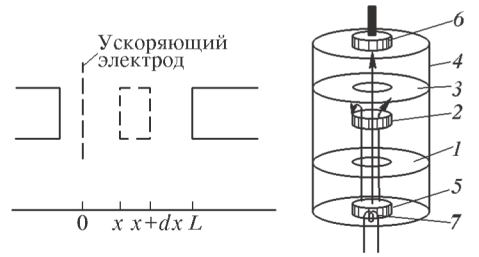
\includegraphics[width = 0.9\textwidth]{Exp setup.png}
    \end{center}
    \caption{Схематическая изображение тиратрона (слева) и его конструкция (справа): $1$, $2$, $3$ -- сетки; $4$ -- внешний металлический цилиндр; $5$ -- катод; $6$ -- анод; $7$ -- накаливаемая спираль}
\end{wrapfigure}
В данной работе для изучения эффекта Рамзауэра используется тиратрон ТГ3-01/1.3Б, заполненный инертным газом. Схематическое изображение тиратрона и его конструкция приведены на рис. 5.

Электроны, эмитируемые катодом тиратрона, ускоряются напряжением $V$ , приложенным между катодом и ближайшей к нему сеткой. Затем электроны рассеиваются на атомах инертного газа (ксенона). Все сетки $1$, $2$, $3$ соединены между собой и имеют одинаковый потенциал, примерно равный потенциалу анода $6$. Поэтому между первой сеткой $1$ и анодом практически нет поля. Рассеянные электроны отклоняются в сторону и уходят на сетку, а оставшаяся часть электронов достигает анода и создает анодный ток $I_a$. Таким образом, поток электронов $N(x)$ на расстоянии $x$ от ускоряющей сетки уменьшается с ростом $x$ от начального значения $N_0$ у катода (в точке $x = 0$) до некоторого значения $N_a$ у анода (в точке $x = L$).

Рассмотрим теперь, какова должна быть реальная вольт-амперная характеристика (ВАХ) тиратрона. Выделим в газе на расстоянии $x$ от катода тонкий слой с площадью поперечного сечения $S$ и толщиной $dx$ (рис. \hyperref[fig: Exp setup]{3}). Этот слой содержит $d\nu = n_a Sdx$ атомов газа. Суммарная рассеивающая поверхность этих атомов (суммарное эффективное сечение рассеяния) $\Delta = \nu\Delta_a$, где $\Delta_a$ -- площадь поперечного сечения атома. Обозначим через $dN$ убыль потока электронов в результате прохождения слоя $dx$, тогда $dN/N(x)$ есть доля рассеянных электронов, или вероятность рассеяния в слое. Для рассеяния электрона в слое необходимо выполнение двух независимых событий -- электрон должен «наткнуться» в слое на
атом, и, кроме того, должен на этом атоме рассеяться. Следовательно, вероятность $dN/N(x)$ рассеяния электрона в слое равна произведению двух вероятностей -- вероятности для электрона в слое $dx$ встретить атом газа и вероятности рассеяния на атоме $w(V)$:
\begin{equation}\label{eq: Scattering probability}
    -\frac{dN}{N(x)} = \frac{\Delta}{S}w(V) = n_a\Delta_a w(V)dx.
\end{equation}

Интегрируя это соотношение от $0$ до $L$ и заменяя поток электронов на ток $I = Ne$, получаем уравнение ВАХ:
\begin{equation}\label{eq: Current-voltage characteristic}
    I_a = I_0e^{-Cw(V)},\; C = L n_a\Delta_a,
\end{equation}
где $I_0 = eN_0$ -- ток катода, $I_a = eN_a$ -- анодный ток.

Согласно классическим представлениям сечение рассеяния электрона на атоме должно падать монотонно с ростом $V$ (обратно пропорционально скорости электрона, т. е. обратно пропорционально квадратному корню из его энергии), а значит, ВАХ будет монотонно возрастающей функцией, как это показано на рис. \hyperref[fig: Current-voltage characteristic]{6а}. По квантовым соображениям вероятность рассеяния электронов и соответствующая ВАХ должны иметь вид, показанный на рис. \hyperref[fig: Current-voltage characteristic]{6б}.
\begin{figure}[H]\label{fig: Current-voltage characteristic}
    \centering
    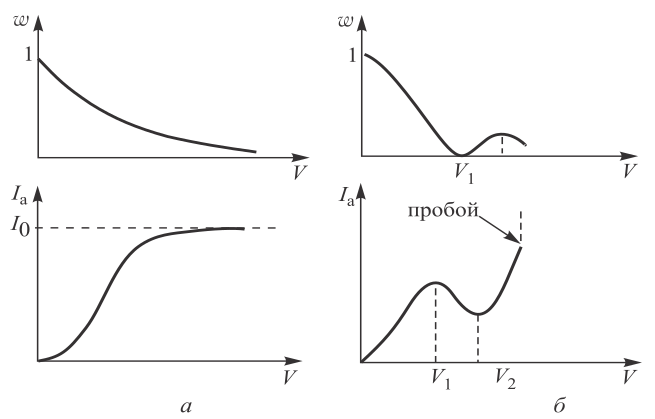
\includegraphics[width = 0.9\textwidth]{Current-voltage characteristic}
    \caption{Качественный вид вероятности рассеяния электрона атомом инертного газа и ВАХ тиратрона при классическом (a) и квантовом (б) рассмотрении}
\end{figure}
Согласно формуле \eqref{eq: Current-voltage characteristic} по измеренной ВАХ тиратрона можно определить зависимость вероятности рассеяния электрона от его энергии из соотношения
\begin{equation}\label{eq: Scattering probability via current}
    w(V) = -\frac{1}{C}\ln\frac{I_a(V)}{I_0}.
\end{equation}

\newpage
\section{Обработка данных}

\subsection{ВАХ тиратрона в динамическом режиме}
Цена деления измерениий в динамическом режиме составляет: $V = 5$ В, $I = 0,1$ А. Максимальное значение ускоряющего напряжения: $V_\text{накал max} = 3,33$ В.
\begin{enumerate}
    \item
    При двух различных ускоряющих напряжениях (одно из которых максимальное для данной установки) измерим напряжения между католом и сеткой, соответствующее первому максимуму и минимумуна осциллограмме, а также оценим напряжение пробоя, соответствующее резкому скачку тока в конце кривой. Результаты приведены в таблице ниже.
    \begin{table}[H]\label{tab: Data dynamic mode}
        \centering
        \begin{tabular}{|
            >{\columncolor[HTML]{FFFFFF}}c |
            >{\columncolor[HTML]{FFFFFF}}c |
            >{\columncolor[HTML]{FFFFFF}}c |
            >{\columncolor[HTML]{FFFFFF}}c |}
            \hline
            {\color[HTML]{000000} $V_\text{накал}$, В} & {\color[HTML]{000000} $V_{max}$, В} & {\color[HTML]{000000} $V_{min}$, В} & {\color[HTML]{000000} $V_\text{пробой}$, В} \\ \hline
            {\color[HTML]{000000} 3,33}   & {\color[HTML]{000000} $-5$}         & {\color[HTML]{000000} $-10$}        & {\color[HTML]{000000} $-17$}                \\ \hline
            {\color[HTML]{000000} 2,65}   & {\color[HTML]{000000} $-4$}         & {\color[HTML]{000000} $-12$}        & {\color[HTML]{000000} $-17$}                \\ \hline
        \end{tabular}
        \caption{Данные измерений в динамическом режиме}
    \end{table}
    Абсолютная погрешность измерения величин $V_{max}, V_{min}$ и $V_\text{пробой}$ составляет $\sigma_V = 0,5$ В. Абсолютная погрешность измерения $V_\text{накал}$ составляет $\sigma_{V_\text{накал}} = 0,1$ В. 
    
    \item 
    Далее везде $r = l/2$ -- радиус электронной оболочки. Приняв, $U_0 = 2,5$ эВ, по данным из таблицы рассчитаем размер электронной оболочки оболочки по формулам \eqref{eq: Max condition} и \eqref{eq: Min condition}:
    \begin{table}[H]\label{tab: l results via U_0}
        \centering
        \begin{tabular}{|
            >{\columncolor[HTML]{FFFFFF}}c |
            >{\columncolor[HTML]{FFFFFF}}c |
            >{\columncolor[HTML]{FFFFFF}}c |}
            \hline
            {\color[HTML]{000000} $V$, В} &
              {\color[HTML]{000000} \begin{tabular}[c]{@{}c@{}}$r$, \AA \\ через $V_{max}$\end{tabular}} &
              \cellcolor[HTML]{FFFFFF}{\color[HTML]{000000} \begin{tabular}[c]{@{}c@{}}$r$, \AA \\ через $V_{max}$\end{tabular}} \\ \hline
            {\color[HTML]{000000} 3,33} &
              {\color[HTML]{000000} $1,19 \pm 0,08$} &
              {\color[HTML]{000000} $1,30 \pm 0,05$} \\ \hline
            {\color[HTML]{000000} 2,65} &
              {\color[HTML]{000000} $1,20 \pm 0,09$} &
              {\color[HTML]{000000} $1,21 \pm 0,04$} \\ \hline
        \end{tabular}
        \caption{Результаты расчёта размера электронной оболочки }
    \end{table}
    Погрешности вычислялись по формуле 
    $$
        \sigma_r^2 = \left(\frac{\partial f(V)}{\partial V}\right)^2 \cdot \sigma_V^2,
    $$
    где $f(V)$ -- одна из функций, выражающих $r$ через $V$: \eqref{eq: Max condition} и \eqref{eq: Min condition}.

    \item
    Теперь рассчитаем то же значение размер электронной оболочки атома, используя выражение \eqref{eq: Atom diameter}:
    \begin{table}[H]\label{tab: l results via V_max and V_min}
        \centering
        \begin{tabular}{|
            >{\columncolor[HTML]{FFFFFF}}c |
            >{\columncolor[HTML]{FFFFFF}}c |}
            \hline
            {\color[HTML]{000000} $V$, В} & {\color[HTML]{000000} $r$, \AA} \\ \hline
            {\color[HTML]{000000} 3,33}   & {\color[HTML]{000000} $1,54 \pm 0,22$}         \\ \hline
            {\color[HTML]{000000} 2,65}   & {\color[HTML]{000000} $1,21 \pm 0,11$}         \\ \hline
        \end{tabular}
        \caption{Результаты расчёта размера электронной оболочки }
    \end{table}
    Погрешности были вычислены по формуле
    $$
        \sigma_r^2 = \left(\frac{\partial f(V_{max}, V_{min})}{\partial V_{max}}\right)^2 \cdot \sigma_{V_{max}}^2 + \left(\frac{\partial f(V_{max}, V_{min})}{\partial V_{min}}\right)^2 \cdot \sigma_{V_{min}}^2,
    $$    
    где $f(V_{max}, V_{min})$ -- функция, выражающая $r$ через $V_{max}$ и $V_{min}$, получающаяся из выражения \eqref{eq: Atom diameter}.

    Результаты вычислений радиуса атомной оболочки по двум различным формулам совпадают друг с другом с неплохой точностью. 

    \item 
    С помощью выражения \eqref{eq: Pootential well depth} рассчитаем глубину потенциальной ямы: 
    $$
        U_0 = (2,4 \pm 0,98) \text{ эВ},
    $$
    $$
        \sigma_{U_0} = \sqrt{\left(\frac{4}{5}\right) + \left(\frac{9}{5}\right)}\sigma_V.
    $$
    
    \item 
    Известно, что различные инертные газы обладают различным потенциалом ионизации: аргон -- $15,8$ эВ, криптон -- $14,0$ эВ, ксенон -- $12,1$ эВ. Самое близкое из них к экспериментально полученному является значения для аргон, отсюда можем сделать вывод, что в данной работе рассеивание электронов происходит на атомах аргона.

    \item 
    Табличное значение радиуса атомной оболочки для атомов аргона: $r_a = 0,71$ \AA, $r_k = 1,06$ \AA, $r_i = 1,54$ \AA, где $r_a$ -- атомный радиус, $r_k$ -- ковалентный радиус, $r_i$ -- ионный радиус атома аргона.   

    \item
    Исследуем поведение системы при поднесении к лампе постоянного магнита. Магнитное поле отклоняет электроны, испытавшие упругое столкновение, а значит и влияет на эффект Рамзауэра. При различных ориентациях магнита на экране осциллографа наблюдается различная картина: меняется (уменьшается) величина анодного тока $I_a$. 
\end{enumerate}

\subsection{ВАХ тиратрона в статическом режиме}
\begin{enumerate}
    \item
    В данном пункте исследуем вольт-амперную характеристику тиратрона в статическом режиме. Для этого снимем зависимость напряжения анод-сетка $U_I$ от падения напряжения между катодом и сеткой $U_V$. В таблице ниже приведены результаты измерений для двух значений напряжения (тока) накала. Погрешность каждого измерения равна $\sigma_V = 0,1$ В.
    \begin{table}[H]\label{tab: U_I via U_v}
        \centering
        \begin{tabular}{|
        >{\columncolor[HTML]{FFFFFF}}c |
        >{\columncolor[HTML]{FFFFFF}}c |
        >{\columncolor[HTML]{FFFFFF}}c |
        >{\columncolor[HTML]{FFFFFF}}c |
        >{\columncolor[HTML]{FFFFFF}}c |
        >{\columncolor[HTML]{FFFFFF}}c |}
        \hline
        {\color[HTML]{000000} №} &
          {\color[HTML]{000000} $U_V$, В} &
          {\color[HTML]{000000} $U_I$, В} &
          {\color[HTML]{000000} №} &
          {\color[HTML]{000000} $U_V$, В} &
          {\color[HTML]{000000} $U_I$, В} \\ \hline
        {\color[HTML]{000000} 1} &
          {\color[HTML]{000000} 0} &
          {\color[HTML]{000000} 0} &
          {\color[HTML]{000000} 8} &
          {\color[HTML]{000000} 6,0} &
          {\color[HTML]{000000} 83,0} \\ \hline
        {\color[HTML]{000000} 2} &
          {\color[HTML]{000000} 2,0} &
          {\color[HTML]{000000} 25,0} &
          {\color[HTML]{000000} 9} &
          {\color[HTML]{000000} 7,0} &
          {\color[HTML]{000000} 77,9} \\ \hline
        {\color[HTML]{000000} 3} &
          {\color[HTML]{000000} 3,0} &
          {\color[HTML]{000000} 49,2} &
          {\color[HTML]{000000} 10} &
          {\color[HTML]{000000} 8,0} &
          {\color[HTML]{000000} 70,0} \\ \hline
        {\color[HTML]{000000} 4} &
          {\color[HTML]{000000} 4,0} &
          {\color[HTML]{000000} 74,5} &
          {\color[HTML]{000000} 11} &
          {\color[HTML]{000000} 8,5} &
          {\color[HTML]{000000} 66,8} \\ \hline
        {\color[HTML]{000000} 5} &
          {\color[HTML]{000000} 4,5} &
          {\color[HTML]{000000} 79,7} &
          {\color[HTML]{000000} 12} &
          {\color[HTML]{000000} 9,0} &
          {\color[HTML]{000000} 64,1} \\ \hline
        {\color[HTML]{000000} 6} &
          {\color[HTML]{000000} 5,0} &
          {\color[HTML]{000000} 82,3} &
          {\color[HTML]{000000} 13} &
          {\color[HTML]{000000} 9,5} &
          {\color[HTML]{000000} 63,1} \\ \hline
        {\color[HTML]{000000} 7} &
          {\color[HTML]{000000} 5,5} &
          {\color[HTML]{000000} 83,2} &
          {\color[HTML]{000000} 14} &
          {\color[HTML]{000000} 10,0} &
          {\color[HTML]{000000} 67,0} \\ \hline
        \end{tabular}
        \caption{Результаты измерения анодного напряжения при $V_\text{накал} = 3,33$ В}
    \end{table}
    \begin{table}[H]\label{tab: V_I via V_v}
        \centering
        \begin{tabular}{|
            >{\columncolor[HTML]{FFFFFF}}c |
            >{\columncolor[HTML]{FFFFFF}}c |
            >{\columncolor[HTML]{FFFFFF}}c |
            >{\columncolor[HTML]{FFFFFF}}c |
            >{\columncolor[HTML]{FFFFFF}}c |
            >{\columncolor[HTML]{FFFFFF}}c |}
            \hline
            {\color[HTML]{000000} №} &
              {\color[HTML]{000000} $U_V$, В} &
              {\color[HTML]{000000} $U_I$, В} &
              {\color[HTML]{000000} №} &
              {\color[HTML]{000000} $U_V$, В} &
              {\color[HTML]{000000} $U_I$, В} \\ \hline
            {\color[HTML]{000000} 1} &
              {\color[HTML]{000000} 0} &
              {\color[HTML]{000000} 0} &
              {\color[HTML]{000000} 10} &
              {\color[HTML]{000000} 7,0} &
              {\color[HTML]{000000} 29,2} \\ \hline
            {\color[HTML]{000000} 2} &
              {\color[HTML]{000000} 2,0} &
              {\color[HTML]{000000} 0} &
              {\color[HTML]{000000} 11} &
              {\color[HTML]{000000} 8,0} &
              {\color[HTML]{000000} 22,9} \\ \hline
            {\color[HTML]{000000} 3} &
              {\color[HTML]{000000} 3,0} &
              {\color[HTML]{000000} 24,5} &
              {\color[HTML]{000000} 12} &
              {\color[HTML]{000000} 8,5} &
              {\color[HTML]{000000} 20,8} \\ \hline
            {\color[HTML]{000000} 4} &
              {\color[HTML]{000000} 3,5} &
              {\color[HTML]{000000} 36,6} &
              {\color[HTML]{000000} 13} &
              {\color[HTML]{000000} 9,0} &
              {\color[HTML]{000000} 18,8} \\ \hline
            {\color[HTML]{000000} 5} &
              {\color[HTML]{000000} 4,0} &
              {\color[HTML]{000000} 42,1} &
              {\color[HTML]{000000} 14} &
              {\color[HTML]{000000} 9,5} &
              {\color[HTML]{000000} 17,6} \\ \hline
            {\color[HTML]{000000} 6} &
              {\color[HTML]{000000} 4,5} &
              {\color[HTML]{000000} 42,2} &
              {\color[HTML]{000000} 15} &
              {\color[HTML]{000000} 10,0} &
              {\color[HTML]{000000} 17,0} \\ \hline
            {\color[HTML]{000000} 7} &
              {\color[HTML]{000000} 5,0} &
              {\color[HTML]{000000} 40,2} &
              {\color[HTML]{000000} 16} &
              {\color[HTML]{000000} 10,5} &
              {\color[HTML]{000000} 16,9} \\ \hline
            {\color[HTML]{000000} 8} &
              {\color[HTML]{000000} 5,5} &
              {\color[HTML]{000000} 37,8} &
              {\color[HTML]{000000} 17} &
              {\color[HTML]{000000} 11,0} &
              {\color[HTML]{000000} 17,2} \\ \hline
            {\color[HTML]{000000} 9} &
              {\color[HTML]{000000} 6,0} &
              {\color[HTML]{000000} 35,3} &
              {\color[HTML]{000000} 18} &
              {\color[HTML]{000000} 12,0} &
              {\color[HTML]{000000} 18,5} \\ \hline
        \end{tabular}
        \caption{Результаты измерения анодного напряжения при $V_\text{накал} = 2,63$ В}
    \end{table}

    \item 
    Далее построим график зависимости $I_a = f(U_V)$. Значения анодного тока можно посчитать из величины соответствующего ему напряжения по формуле $I_a = U_I / R_0$, где $R_0 = 100$ кОм -- сопротивление, включённое в цепь анода. 

    \item 
    Используя формулу \eqref{eq: Max condition via n}, выведем зависимость $E_n$ -- $n$-го максимума от $E_1$ и $n$:
    $$
        \sqrt{\frac{2m(E + U_0)}{\hbar^2}}l = \pi n \Rightarrow
    $$
    $$
        E_n = n^2(E_1 + U_0) - U_0
    $$
    Используя формулу выше оценим $E_2 > 15$ эВ -- при таких энергиях происходит ионизация газа и, как следствие, пробой, поэтому измерить второй максимум не удаётся.

    \item 
    Построим график зависимости вероятности рассеяния $w$ от величины $-\ln\frac{I_a(V)}{I_0}$, где $I_0$ -- значение анодного тока, при котором наблюдается первый максимум. $I \propto V \Rightarrow$ будем строить график зависимости $w$ от $-\ln\frac{V_I}{V_0}$.
    
\end{enumerate}

\section{Вывод}
В данной работе исследовалось явление эффекта Комптона. В результате удалось:
\begin{itemize}
    \item
    измерить зависимость вероятности рассеяния электрона на атомах инертного газа (аргона) от его энергии. Получить экспериментально характерные максимум и минимум вероятности рассеяния в диапазоне энергий $0-12$ эВ.
    
    \item
    различными способами оценить характерный радиус атома аргона. Результаты с неплохой точностью совпали с табличными значениями.

    \item
    оценить глубину потенциала атома аргона в приближении прямоугольной потенциальной ямы.
    
\end{itemize}

\newpage
%%%%%%%%%%%%%%%%%%%%%%%%% Графики
\begin{figure}[H]\label{fig: I_a(U_V)}
    \centering
    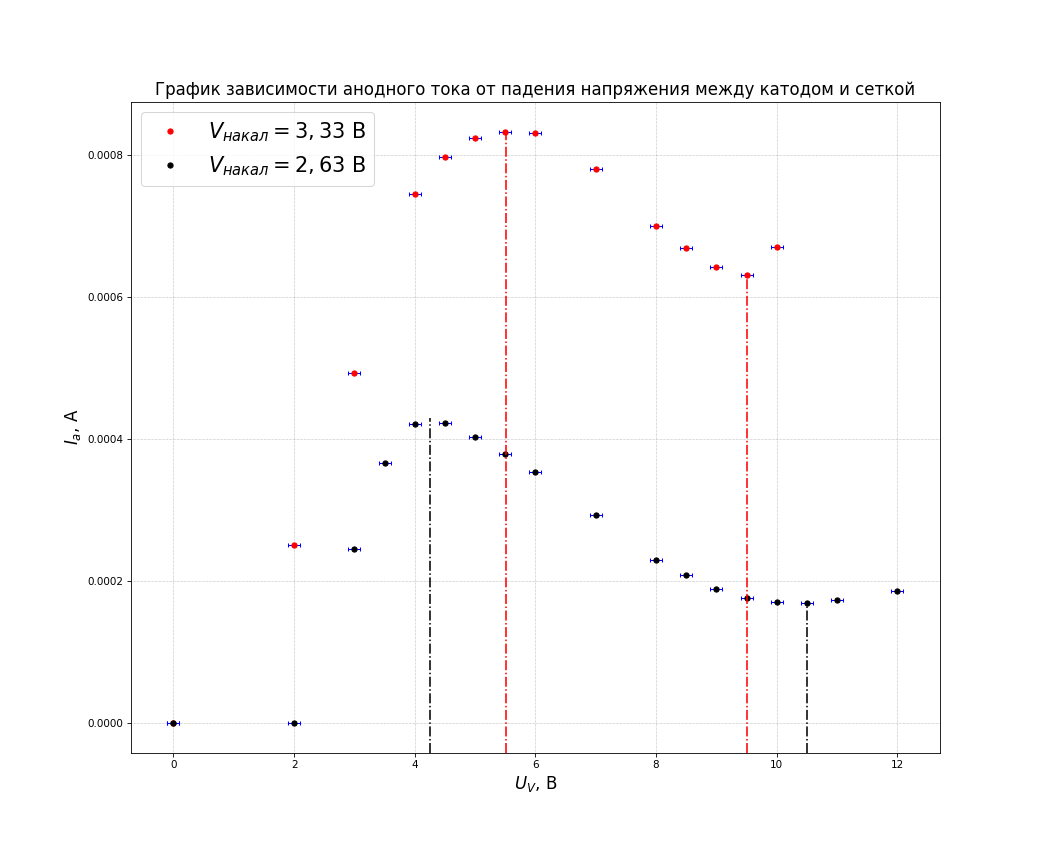
\includegraphics[width = \textwidth]{I_a(U_V).png}
\end{figure}
Из графика получим новые значения для $V_{min}$, $V_{max}$. По этим значениям пересчитаем радиус атома:
\begin{table}[H]\label{tab: Data dynamic mode corrected}
    \centering
    \begin{tabular}{|
        >{\columncolor[HTML]{FFFFFF}}c |
        >{\columncolor[HTML]{FFFFFF}}c |
        >{\columncolor[HTML]{FFFFFF}}c |
        >{\columncolor[HTML]{FFFFFF}}c |}
        \hline
        {\color[HTML]{000000} $V_\text{накал}$, В} & {\color[HTML]{000000} $V_{max}$, В} & {\color[HTML]{000000} $V_{min}$, В} \\
        \hline
        {\color[HTML]{000000} 3,33}   & {\color[HTML]{000000} $-5,51$}         & {\color[HTML]{000000} $-9,5$} \\
        \hline
        {\color[HTML]{000000} 2,65}   & {\color[HTML]{000000} $-4,25$}         &{\color[HTML]{000000} $-10,5$} \\
        \hline
    \end{tabular}
    \caption{Данные из графика в статическом режиме}
\end{table}
$$
    \sigma_V = 0,1 \text{ В}    
$$
\begin{table}[H]\label{tab: l results via U_0 corrected}
    \centering
    \begin{tabular}{|
        >{\columncolor[HTML]{FFFFFF}}c |
        >{\columncolor[HTML]{FFFFFF}}c |
        >{\columncolor[HTML]{FFFFFF}}c |}
        \hline
        {\color[HTML]{000000} $V$, В} &
            {\color[HTML]{000000} \begin{tabular}[c]{@{}c@{}}$r$, \AA \\ через $V_{max}$\end{tabular}} &
            \cellcolor[HTML]{FFFFFF}{\color[HTML]{000000} \begin{tabular}[c]{@{}c@{}}$r$, \AA \\ через $V_{max}$\end{tabular}} \\ \hline
        {\color[HTML]{000000} 3,33} &
            {\color[HTML]{000000} $1,15 \pm 0,04$} &
            {\color[HTML]{000000} $1,33 \pm 0,02$} \\ \hline
        {\color[HTML]{000000} 2,65} &
            {\color[HTML]{000000} $1,18 \pm 0,04$} &
            {\color[HTML]{000000} $1,28 \pm 0,02$} \\ \hline
    \end{tabular}
    \caption{Результаты расчёта размера электронной оболочки по графику}
\end{table}
\begin{table}[H]\label{tab: l results via V_max and V_min corrected}
    \centering
    \begin{tabular}{|
        >{\columncolor[HTML]{FFFFFF}}c |
        >{\columncolor[HTML]{FFFFFF}}c |}
        \hline
        {\color[HTML]{000000} $V$, В} & {\color[HTML]{000000} $r$, \AA} \\ \hline
        {\color[HTML]{000000} 3,33}   & {\color[HTML]{000000} $1,72 \pm 0,11$}         \\ \hline
        {\color[HTML]{000000} 2,65}   & {\color[HTML]{000000} $1,37 \pm 0,06$}         \\ \hline
    \end{tabular}
    \caption{Результаты расчёта размера электронной оболочки по графику}
\end{table}

\begin{figure}[H]\label{fig: w(V) first V}
    \centering
    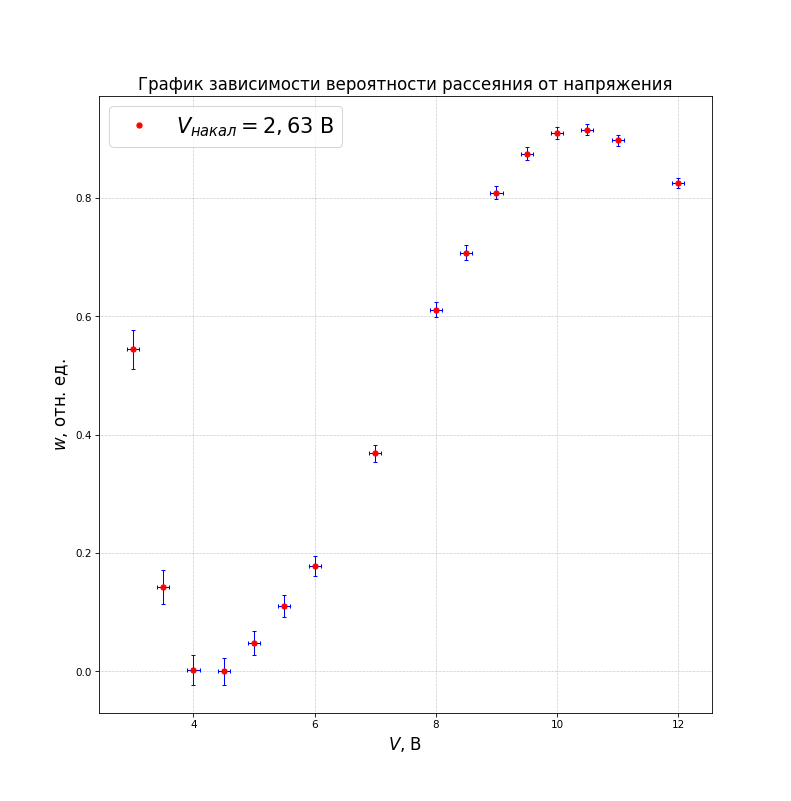
\includegraphics[width = \textwidth]{w(V)first.png}
\end{figure}

\begin{figure}[H]\label{fig: w(V) second V}
    \centering
    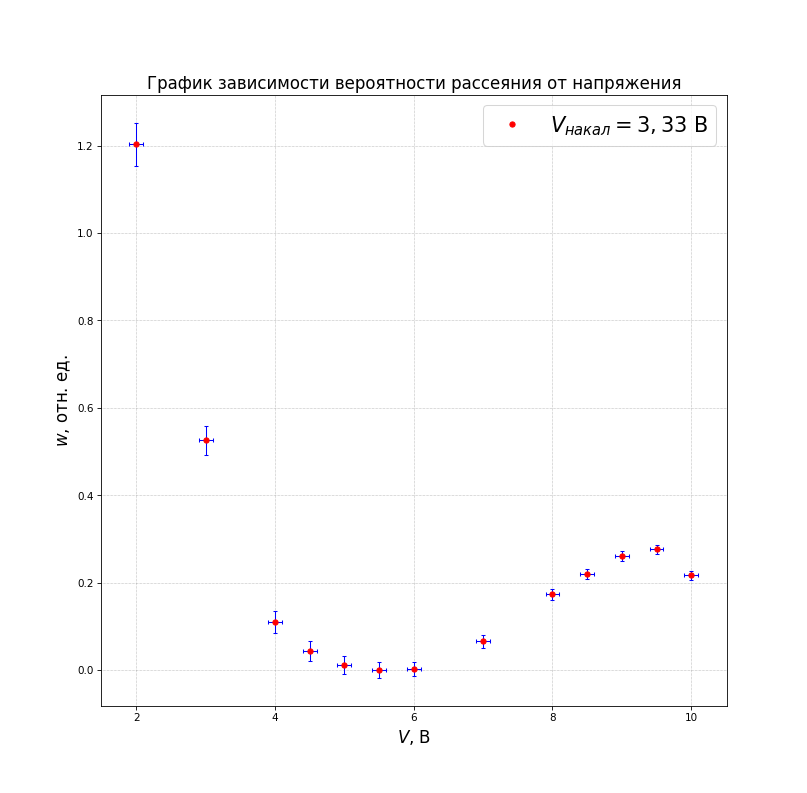
\includegraphics[width = \textwidth]{w(V)second.png}
\end{figure}

%%%%%%%%%%%%%%%%%%%%%%%%%
\end{document}
